\documentclass[UTF8,oneside]{ctexbook}

\usepackage[titles]{tocloft} % 目录
\usepackage[colorlinks,linkcolor=blue]{hyperref} % 超链接
\usepackage{graphicx} % An example of a floating figure using the graphicx package.
\usepackage{animate} % 动画
\usepackage{enumerate} % 列表
\usepackage{fancyhdr} % 页眉页脚
\pagestyle{fancy}
\usepackage{xpinyin} % 注音
\usepackage[]{appendix}

\title{\Huge{A NOTE {\itshape of} MASTER}\\
\Huge{菜鸟硕士手册}\\
\large{V1.0}}
\author{\href{https://github.com/lonelybag?tab=repositories}{\Large{@LonelyBag}}\\ {\itshape \large{Edite by \href{https://mirrors.tuna.tsinghua.edu.cn/CTAN/systems/texlive/Images/}{\LaTeX}}}}

\begin{document}
% ----------- 封面 ---------------
\frontmatter
\maketitle

% \begin{center}  % 居中
% 	\quad \\
% 	\vspace{3cm}
% 	\hspace{3cm}\Huge{A NOTE {\itshape of} MASTER}\\
% 	\hspace{3cm}\Huge{菜鸟硕士手册} \\
% 	\hspace{3cm}\large{V1.0} \\
% 	\vspace{5cm}
% 	\hspace{3cm}\href{https://github.com/lonelybag/Latex_lonelybag}{\Large{@LonelyBag}}\\
% 	\vspace{0.5cm}
% 	\hspace{3cm}\Large{2018.3.2}
% 	\clearpage  % 清除当页页码
% \end{center}

\begin{center}  % 居中
	\quad \\
	\vspace{5cm}
	\LARGE{如果说我比别人看得更远,那是因为我站在巨人的肩膀上}\\
	% \LARGE{上下四方曰宇,古往今来曰宙}
\end{center}
\thispagestyle{empty}
% ----------- 目录 ---------------
\tableofcontents

\mainmatter
% ----------- 正文 ---------------
\chapter{试着不虚此行}
硕士期间,我听到身边同学说的最多的就是叹气。 不满意、不理想好像成了日常的生活状态,
\section{假如重新来过}
假如我回到了三年前再次读研。我会这样度过:
\begin{itemize}
	\item 研一上,认真学好数值分析、矩阵论、智能控制理论、电力电子、DSP以及文献检索(比较有代表性的,不代表其他不重要)。原因:数值分析和矩阵论是一切仿真软件内核的数学基础;智能控制理论涉及到了人工神经网络的基本原理,而它是未来的必然趋势,此外书中提到的算法都可以解决优化问题,如:电路拓扑的构建、电路元件参数的调整、线圈形状的优化等等。。。电力电子电路和DSP的结合是除了仿真外验证思路的最优实现方案;文献检索,可能是硕士期间最重要、也最值得花时间研究的课。
	\item 研一下,只做两件事。第一:系统地学习MATLAB+Simulink、COMSOL或Ansys、DSP、Altium Designer、ADS或Multism、Latex+git+vscode、Rhino或3DSMAX、PS或Adobe Illustrator。第二:整理近两年的论文。
	\item 研二上(开题10月底),精进MATLAB+Simulink、COMSOL或Ansys、DSP、Altium Designer、ADS或Multism、Latex+git+vscode,并着手仿真实验+写论文引言。
	\item 研二下(中期5月底),完成实验,完成论文并在11月份前投出。
	\item 研二上,着手第二篇论文,在9月份前投出。
	\item 研三上(毕业答辩1月底),完成毕业论文。
\end{itemize}

这将是异常\xpinyin{丰}{tong4}\xpinyin{富}{ku3}的经历,如果坚持下来,你的人生可能就会因此\xpinyin{改}{tu1}\xpinyin{变}{ding3}。


\chapter{快速抓住研究热点}
研究热度往往体现在论文的发表数量中,但是一个领域中的主要研究方向却往往很难仅通过阅读论文而获得全面认识。换句话说,统计论文中的研究方向远比统计发表数量重要。为了解决这一问题,研究人员也提出了若干解决方案。

\section{传统方式}
词典,是语言学家针对特定语言而将常见字词按照一定的逻辑编纂起来的文本工具。科学家也有自己的词典,他们针对某一特定研究领域对热点论文进行总结归纳并提出相应见解,最终以论文的形式发表,这就是文献综述。

通过阅读文献综述,可以快速地对所关注的研究领域形成大致了解,而这也是快速抓住研究热点的传统方式。通过限定检索词可以较为有效地检索该类型的文章,对于英文文献,其检索词可以选择如下几种:
\begin{itemize}
	\item Review
	\item Challenge
	\item Survey
	\item Statement
	\item ... ...
\end{itemize}

这样,再加上一些限定词(如:WPT)就可以有效地检索出特定研究领域的文献综述。但是,这样检索出的文献往往比较松散,并且会使我们忽略一些更有价值的paper。因此,有时(甚至往往)会采用辅助工具进行这项工作。

\section{辅助工具}
为了快速地了解一个领域的研究热点,仅仅通过 {\bf 关键词检索 - 论文下载 - 阅读 - 二次检索} 这类流程是不能达到“快速”的要求的,真正有效的方法是借助论文分析工具,这类工具一般有如下特点:

\begin{itemize}
	\item 可以分析大量文献间的交叉检索关系
	\item 结果可视化
	\item 多功能
\end{itemize}

常用的辅助工具有:\href{https://zhuanlan.zhihu.com/p/20902898}{HistCite Pro 2.1} 以及 \href{https://zhuanlan.zhihu.com/p/30970993}{VOSviewer}、Citespace。这两种工具的最大区别就是HistCite Pro 2.1仅支持英文文献,但VOSviewer不仅支持英文还支持中国知网导出的中文文献。笔者只用过HistCite Pro 2.1,如果读者希望对中文文献也进行处理,可以参考\href{https://www.jianshu.com/p/e20f3f1d17d8}{这个})。下面我通过若干gif对软件的使用进行介绍。
\subsection{安装}
安装就不赘述了,参考\href{https://zhuanlan.zhihu.com/p/20902898}{这里}就够了。
\subsection{导出文献}
这一步是初学者最容易出现差错的地方,这是因为HistCite Pro 2.1对源数据的格式要求非常严谨,而且它仅支持由Web of Science导出的文献格式。下面我通过Step-by-step的方式展示如何从WOS导出符合要求的格式。

第一步:选择检索{\bf 数据库}并给定检索词,一般首次使用需要我们对整个领域有一个宏观认识,因此检索词可以非常概括,比如我使用的wireless power,如图\ref{fig:1}。

\begin{figure}[!htb]
	\centering
	\animategraphics[autoplay, loop , width=0.9\linewidth]{8}{Figure//WOSsearch//10}{01}{80}
	\vspace{-0.3cm}
	\caption{WOS检索关键词:wireless power}\label{fig:1}
\end{figure}

第二步:选择正确格式,下载,如图\ref{fig:2}所示。值得注意的是,WOS仅支持一次性导出500篇文献,所以更多的文献需要多次下载,这步完成后会获得一个包含所有文献检索信息的txt文件。

\begin{figure}[!htb]
	\centering
	\animategraphics[autoplay, loop , width=0.9\linewidth]{8}{Figure//WOSdownload//00}{01}{98}
	\vspace{-0.3cm}
	\caption{WOS下载特定格式检索结果}\label{fig:2}
\end{figure}

\subsection{文献分析}
将下载获得的所有txt移动至TXT文件夹,然后打开main.exe,此时输入1并回车,软件将自动打开程序界面,接着点击gragh maker,我们就会获得文献之间的引用网络,文献由节点表示,所有的节点自上而下按照时间顺序排列,之间的引用和被引关系由连接的线条表示。修改count将对分析的文献数量进行控制,一般来说,取得大一点可以获得更多的信息,如图\ref{fig:3}所示。

\begin{figure}[!htb]
	\centering
	\animategraphics[autoplay, loop , width=0.9\linewidth]{8}{Figure//Hmaker//00}{01}{73}
	\vspace{-0.3cm}
	\caption{HistCite Pro 2.1操作}\label{fig:3}
\end{figure}


注意到,select by一栏有两个选项:LCS和GCS,LCS是Local Citation Score的缩写,代表某篇文献在本地数据集(也就是我们所下载的txt集合)的总被引次数,而GCS是Global Citation Score的缩写,代表在WOS数据库中的总被引次数。一般来说,由于本地数据集是根据我们的关键词获得的,因此LCS排名更能够反映某一学科的发展。此外,还有两个参数会出现在浏览器界面,CR和LCR,分别是Cited references和local cited references的缩写,代表对WOS数据库和本地数据库文献引用的数量。这里,CR越高(一般以50篇为标准)则表示该文献越可能是综述性文献,这样就可以方便地追根溯源,清晰地看到一个学科乃至一个领域的发展脉络,一个典型的发展脉络可以参考图\ref{fig:typical_trace}(完整版请\href{https://raw.githubusercontent.com/lonelybag/Latex_lonelybag/V1.0/Script/002_NOTE_of_MASTER/Figure/typical_trace_full.jpg}{移步})。

\begin{figure}[!htb]
	\centering
	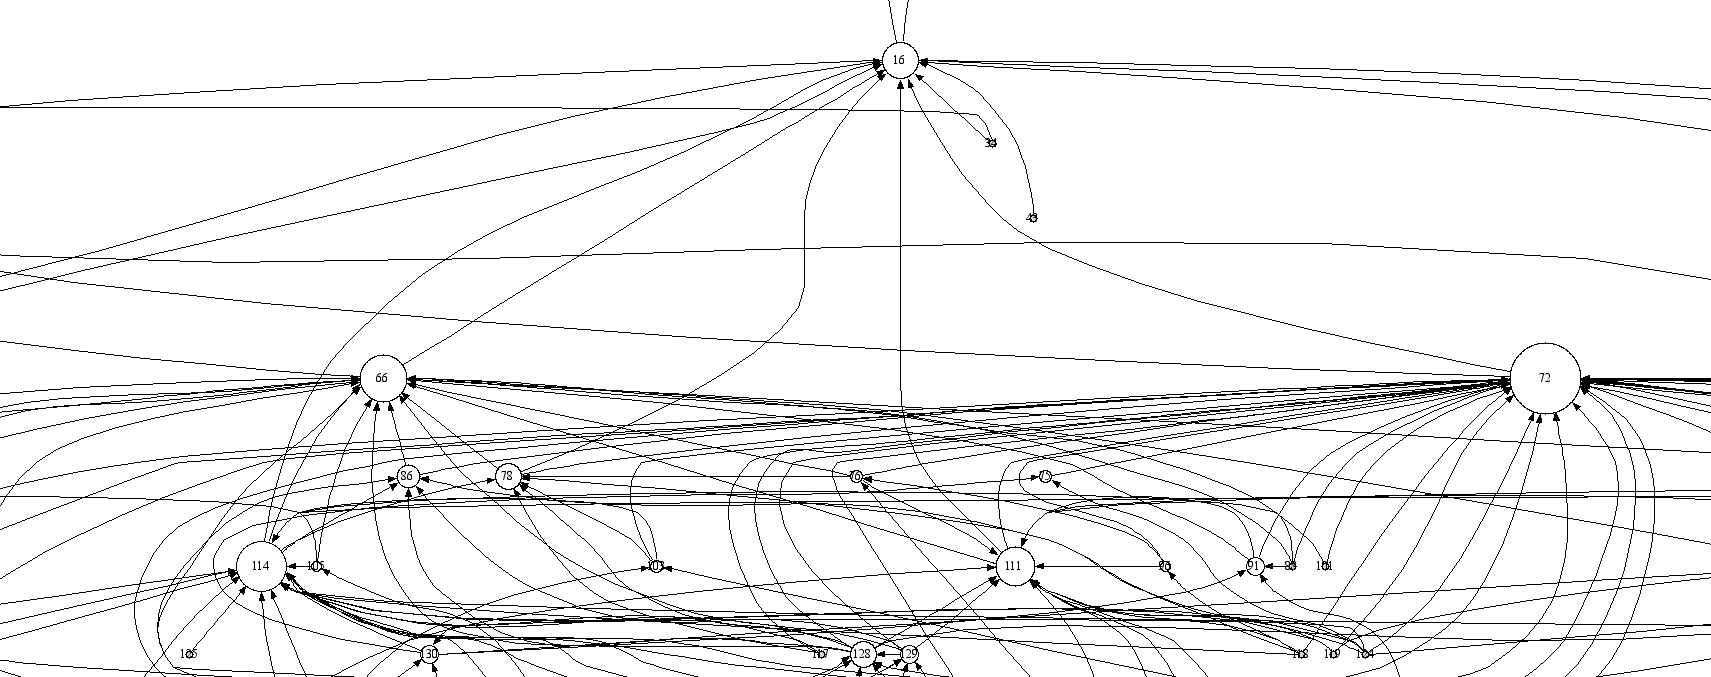
\includegraphics[width=1\linewidth]{Figure/typical_trace.JPG}
	\vspace{-0.3cm}
	\caption{一个示例}\label{fig:typical_trace}
\end{figure}

可以看出,文献16显然是这个领域的开创性论文,随着时间的推移又分裂为两个分支,接着又发展为多个分支。通过阅读关键节点论文不仅可以快速了解这个领域的发展脉络,甚至还可以看出:

\begin{itemize}
	\item 研究之初,两个小方向是经过试探却又半途而废的
	\item \href{https://raw.githubusercontent.com/lonelybag/Latex_lonelybag/V1.0/Script/002_NOTE_of_MASTER/Figure/typical_trace_full.jpg}{完整版图片}右侧出现了两个领域的交叉,这里往往是研究思路的“不老泉”
	\item \href{https://raw.githubusercontent.com/lonelybag/Latex_lonelybag/V1.0/Script/002_NOTE_of_MASTER/Figure/typical_trace_full.jpg}{完整版图片}最左侧有一个研究历程非常持久的小分支,这可能是某个专家的“独门秘籍”
	\item \href{https://raw.githubusercontent.com/lonelybag/Latex_lonelybag/V1.0/Script/002_NOTE_of_MASTER/Figure/typical_trace_full.jpg}{完整版图片}右侧还有一个完全没有关联的领域,虽然在2013年后就没有产出了,但是这并不一定意味着研究的停滞,也有可能是研究成果实现了产业化,被大佬们拿去挣钱了。。。
	\item 。。。 。。。
\end{itemize}

所以,这个方法不仅仅可以帮助我们找文献,更重要的是带给了我们关于这项研究的历史发展历程,带给了我们冰冷研究的人文情怀,我们甚至可以想象出,那位开山鼻祖级别的大佬在当时仅仅是一位年轻博士生的时候的艰苦、悲痛、遇到机遇时狂喜、受挫后的再一次站立、以及功成名就之后的平凡和悠闲。。。

因此,每一张图都可以说是一位科学家的成名史、一个领域的发展史、以及整个人类文明的历史。

所以,为什么不试试\href{https://zhuanlan.zhihu.com/p/20902898}{它}或\href{https://zhuanlan.zhihu.com/p/30970993}{它}呢?

\chapter{罗马是如何建成的}
\section{是时候学点管理学了}
\subsection{什么是工作流}
我平常接触github比较多(一个著名的代码托管网站,这是\href{https://github.com/lonelybag?tab=repositories}{我的主页})。我发现,在进行大多数的代码项目前,大家都会提到一个叫做workflow(可以翻译为工作流)的东西。经过了解后,我发现这个东西非常强大,其本质就是所谓的“思路”或者“技术路线”,并且除了给出方法论以外,它还告诉了我们如何进行团队协作。

workflow源于Github,因此先对Github进行介绍。Github由Linus Torvalds编写的版本控制工具Git发展而来,这两样工具的发明最初仅是为了服务于\href{https://github.com/torvalds/linux}{Linux}项目的开发。Linux作为一个操作系统内核,一个人不可能进行维护,而Github的出现,使得世界范围的代码爱好者可以共同维护一个项目,而这在以前是绝无可能的。

如果说Github提供了一个巨型的合作平台,那么workflow则提供了开发者们共同协作的机制。一个典型的github workflow如图\ref{fig:workflow}所示。

\begin{figure}[!htb]
	\centering
	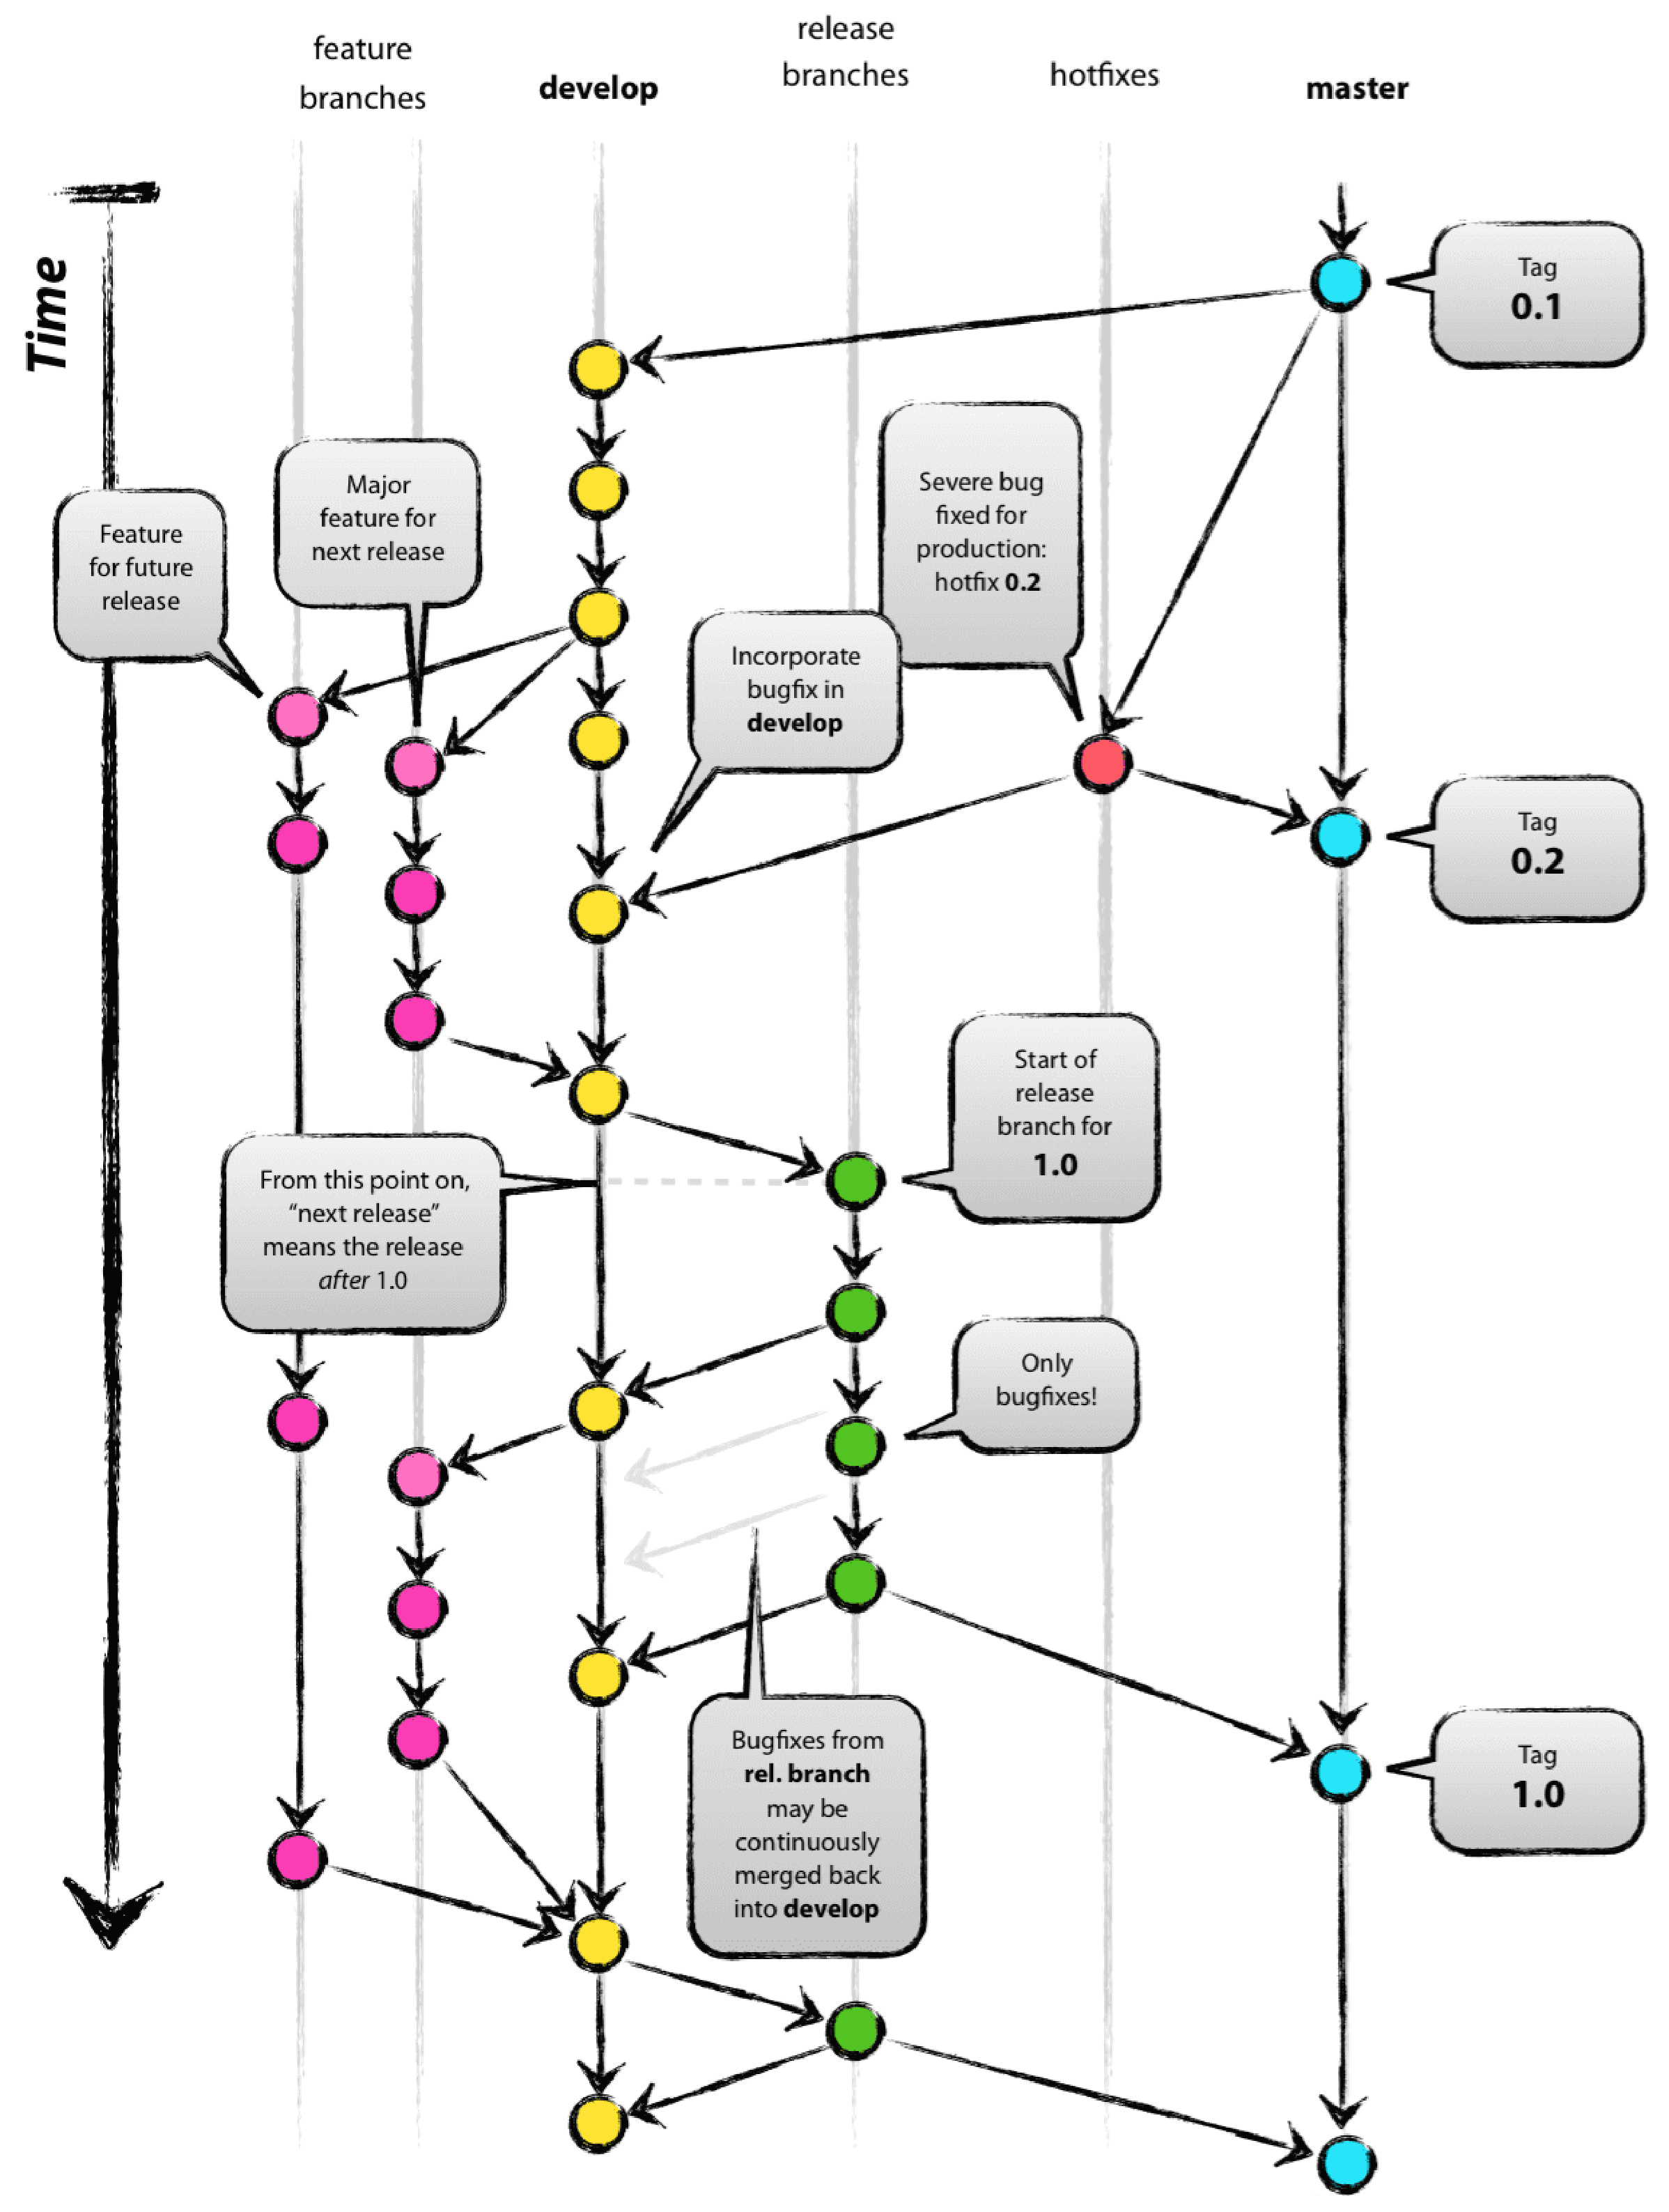
\includegraphics[width=1\linewidth]{Figure/workflow.pdf}
	\vspace{-0.3cm}
	\caption{workflow}\label{fig:workflow}
\end{figure}

\subsection{工作流与科研}
看完这张图大家是不是就明白了,APP中的版本标签V1.1,V1.2其实就是这么来的。

\section{理论分析}
\subsection{为什么要建数学模型}
大到宇宙洪荒,小到亚原子领域,与人类活动相关的一切都有数学模型。那么,为什么要研究呢?我觉得其一是为了控制,其二是为了更加本质地理解现象以得到有用的结论。

\subsection{真实与仿真}
数学模型的建立,使得我们可以通过量化的方式对系统进行控制与优化,

\footnote{钱学森有一个世纪之问:“为什么中国出不了诺贝尔奖”,我自己有一个解答,不是从教育的角度,而是从国人与老外的思考方式的差异,大家有兴趣可以看看\ref{fuluA}。}

\section{实验验证}

\chapter{文献写作}
\section{写作工具}
\section{写作流程}
\section{常用软件}
在我看来,若要完成一项研究报告,我们需要完成以下(或者其中几项)任务:
\begin{itemize}
	\item 仿真
	\item 数据处理
	\item 数据可视化
	\item 算法或者设计优化流程可视化
	\item 实验系统拟物化简图
	\item 电路拓扑绘制
\end{itemize}
\subsection{仿真}
从不同理论的角度分类,可以将仿真分为电路仿真、电磁场仿真以及控制理论仿真。
所谓电路仿真,指可以对等效电路模型进行仿真的软件,一般有如下需求时需要借助该类软件:对所推导的数学模型进行正确性检验、通过快速在线地调节电路参数找创新点、
对由其他理论(如电磁场理论)获得的结论进行验证、控制算法的检验等。
常用的电路仿真软件有:Simulink、ADS、Spice、SABER、Cadence Spectre、Mentors ModelSim、Multisim、proteus(可与keil联调)、Infineon Designer、ADS或Multism、pspice(已经并入orcad)、

芯片检索:alldatasheet、datasheetarchive、\href{http:\\datasheet.eeworld.com.cn}{电子工程世界}


\section{参考文献}


\chapter{上帝说:要有神器}
我只用过其中的一部分,另一部分是还没有时间尝试的,我用\underline{斜体$+$下划线}表示\textbf{没有}用过的。
\section{卸载类}
\begin{itemize}
	\item \href{https://geekuninstaller.com/download}{Geek}
	\item Revo Uninstaller Pro
	\item \href{https://lockhunter.com}{lockhunter}用于删除时出现该文件正在占用
	\item 
\end{itemize}

\section{杀毒、垃圾整理、系统优化}
\begin{itemize}
	\item 火绒
	\item ccleaner
	\item \href{https://bitsum.com}{Process Lasso}用于优化系统进程,提高运行速度
	\item FastCopy 文件复制加速软件
	\item Listery
	\item 傲梅分区助手
\end{itemize}

\section{制作文档类}
\begin{itemize}
	\item GIF录屏:LICEcap、ScreenToGif(2M)、Ocam(10Mb)
	\item Gif转换为图片 Ulead GIF Animator
	\item PDF转换为矢量图片 Inkscape
	\item Vscode
	\item texlive
	\item Atom
	\item 思维导图:幕布(34Mb)
	\item 截屏 FastStone Capture、Snipaste
	\item 快速浏览 QuickLook、seer
	\item \href{https://picpick.app/zh/}{PicPickp屏幕取色}
	\item \href{https://otp.landian.vip/zh-cn/}{office365}
\end{itemize}

\section{下载}
\begin{itemize}
	\item JDownloader2
	\item Send Anywhere
	\item Xtreme Download Manager
	\item \href{https://www.freedownloadmanager.org/}{FDM}
	\item \href{https://webtorrent.io}{磁力在线播放}
\end{itemize}

\section{Chrome插件类}
\begin{itemize}
	\item 油猴脚本
	\item VPN
	\item Listen1
	\item Kopernio
\end{itemize}

\section{常用网站}
\begin{itemize}
	\item \href{https://www.3d66.com/popsoft_26.html}{软件下载}包括但不限于:3DSMAX,AutoCAD,PS,Rhino,Maya,AI。。。
	\item \href{http://gitbook.liuhui998.com/index.html}{Git学习}
	\item \href{http://www.latexstudio.net/archives/6888.html}{GB/T7714-2015参考文献格式}毕业论文有用
	\item \href{http://www.xuexiniu.com/forum.php?mod=forumdisplay&fid=102&filter=typeid&typeid=1}{犀牛技巧}
	\item \href{https://www.52pojie.cn/thread-716675-1-1.html}{一个电路仿真APP}特点是,可以看到电流
	\item \href{http://naotu.baidu.com/file/97d9cd5ca30672903a3e3321e62c6ed8}{百度脑图}、\href{https://github.com/lonelybag/pwc}{Xmind}
	\item \href{https://mm.edrawsoft.cn/map.html?obj=wxoa3v5wBLcpmgCifx59_Uzk5X4qHU/Personal/未命名文件.emmx}{思维导图}更专业一点
	\item \href{https://www.processon.com/login;jsessionid=022BCDCA031DD3C240BE7FD87D942F03.jvm1?backUrl=/diagraming/5be7a513e4b0d74dc539976e}{流程图}
	\item \href{https://ankiweb.net/shared/decks/}{记忆神器}
	\item \href{https://tool.lu}{程序员的工具箱}
	\item \href{http://www.ytube.win}{下载youtube视频}缺点是不带字幕
	\item \href{https://cloudconvert.com/gif-to-mp4}{Gif2MP4}
	\item \href{https://cn.office-converter.com/FIG-to-EPS}{Fig2EPS}
	\item \href{https://www.photopea.com}{在线PS}
	\item \href{https://uzer.me/u/signin}{在线office,PS,AI,MATLAB等}
	\item \href{https://bigjpg.com}{无损放大图片}
	\item \href{https://leetcode.com}{Leetcode}以及\href{https://www.lintcode.com/zh-cn/accounts/signup/}{lintcode} 代码训练平台
	\item \href{https://www.slant.co}{帮助我们做决策}
	\item \href{http://www.pythontutor.com}{python代码在内存中是如何执行的}
	\item \href{https://www.appinn.com/category/windows/}{小众软件}
	\item \href{https://www.remove.bg}{自动抠图}
	\item \href{https://algorithm-visualizer.org}{算法运行可视化}
	\begin{itemize}
		\item \href{http://detexify.kirelabs.org/classify.html}{手写LaTeX符号}
		\item JabRef
		\item Excel2Latex
		\item MetaPOST
		\item Gnuplot
	\end{itemize}
	\item \href{https://learngitbranching.js.org/?demo}{动画学习Git}
	\item \href{https://www.stateoftheart.ai}{MIT整理的关于神经网络的论文}
	\item \href{https://github.com/lonelybag/pwc}{神经网络论文以及源代码}
\end{itemize}

\section{英语写作}
\begin{itemize}
	\item 英语语法检查 \href{https://languagetool.org}{LanguageTool}、\href{https://www.grammarcheck.net}{grammercheck}、\href{https://www.scribens.com}{scribens}、\href{https://www.grammarly.com}{grammerly}、\href{https://www.nounplus.net}{nounplus}
	\item 查介词搭配等等 \href{https://www.english-corpora.org/coca/}{ Corpus of Contemporary American English}、\href{https://www.lintcode.com}{linggle}
	\item 近义词 \href{https://www.thesaurus.com}{theasurus}
\end{itemize}

\section{最小配置}
在此,给出一个我常用的最小配置:

\begin{table}[!bt]
	\renewcommand{\arraystretch}{1.2} %可以让行显得更加宽敞
	\caption{最小配置}\label{tab:mini_configure}
	\vspace{-0.2 cm}
	\centering
	\resizebox{0.9\columnwidth}{!}{ %使得表格能够自动缩放每行长度
		\begin{tabular}{l l l}
			\hline \hline						   \\ [-3 mm]
			用途              & 软件                                                                                     \\
			\hline								   \\ [-3 mm]
			卸载软件          & \href{http://www.xue51.com/soft/11977.html}{Revo Uninstaller Pro}                        \\
			文档撰写          & \href{https://mirrors.tuna.tsinghua.edu.cn/CTAN/systems/texlive/Images/}{\LaTeX} 和 WORD \\
			撸代码            & \href{https://code.visualstudio.com}{Vscode}                                             \\
			版本管理+团队协作 & \href{https://git-scm.com}{Git}                                                          \\
			PDF阅读           & \href{https://www.tracker-software.com/product/pdf-xchange-editor}{PDF-XChange Editor}   \\
			视频播放          & \href{http://potplayer.daum.net/?lang=zh_CN}{PotPlayer}                                  \\
			文件搜索          & \href{https://www.listary.com}{Listery}                                                  \\

			\hline \hline
		\end{tabular}
	}
	\vspace{-0.5cm}
\end{table}

\section{绘图}
\begin{itemize}
	\item Origin
	\item Sigmaplot
	\item Graphpad
	\item Photoshop
	\item Adobe Illustrator
	\item C4D
	\item 3ds MAX
	\item geogebra(开源)
	\item \href{https://affinity.serif.com/zh-cn/designer/}{affinity designer}
	\item SPSS
	\item NVivo
	\item 
\end{itemize}

\section{其他}
\begin{itemize}
	\item Send Anywhere
	\item \href{https://www.scimagojr.com}{SCI期刊}
	\item \href{http://libgen.io}{免费专业书籍}
\end{itemize}

\backmatter
\chapter*{跋}\addcontentsline{toc}{chapter⟩}{跋}
讲几个事例作为结束。

\subsection*{热爱}
时常有人问我:“你怎么会有时间去学那么多东西的?”。其实很简单,因为热爱。

\subsection*{持久的输出}
知乎上有一个问题,苹果公司有哪些黑科技?其中一个回答的答案是iPhone一代。2007年1月,苹果公司发布了被后人称为“重新定义了手机”的iPhone一代,自此开始了长达十年的封神之路。作为历史上市值第一个超过万亿美元的科技公司,它的成功也让很多人萌发了试图复制这一商业成功的欲望,当然他们并未成功,因为十年后的今天苹果依然是第一。很多人将苹果的成功归功于乔布斯,这种想法其实很愚蠢。那么到底是什么造就了它的成功呢?

如果大家读过《乔布斯传》就会了解到,2007年发布的iphone一代,其实早在5年前就已经开始准备了。那就是2002年,还是各种翻盖、滑盖、旋转盖手机迭起的风云时代。。。

我们输的不冤枉。对手感觉到的“黑科技”,其实对自己不过是孕育和必然。

\subsection*{人为什么活着?}
为了心中的梦想。

\vspace{2cm}
总结起来就是三句话:试着让内心去做决策,时刻雕琢自己以及捍卫梦想。

\hspace{4cm}\\
\noindent2019毕业前夕\\
于天津工业大学 \quad 电气学院







\chapter*{附录 A}\addcontentsline{toc}{chapter⟩}{附录 A}\label{fuluA}
如果大家看过《降临》这部电影就会了解,语言决定了(或者反映了)一个人的思考方式,电影中的外星人具有非线性的高维语言能力,没有时间空间的线性概念,这也是电影中人类语言学家不能理解外星人文字的症结。我们可以仿照着看一下汉语与英语的差别,如表\ref{tab:compareCandE}:

\begin{table}[!htb]
	\renewcommand{\arraystretch}{1.3} %可以让行显得更加宽敞
	\caption{中英对比}\label{tab:compareCandE}
	\centering
	\vspace{0.2cm}
	\resizebox{0.3\columnwidth}{!}{
		\begin{tabular}{ccc} % 通过添加 | 来表示是否需要绘制竖线
			\hline  % 在表格最上方绘制横线
			对比       & 汉语 & 英语 \\
			\hline  %在第一行和第二行之间绘制横线
			奇怪的量词 & 少   & 多   \\
			感情色彩   & 委婉 & 直接 \\
			时态       & 无   & 有   \\
			\hline % 在表格最下方绘制横线
		\end{tabular}
	}
\end{table}

可以看出,中国人的语言是弱化量词而强化情感的,我们作画作诗也是这样,总是注重写意而避免写实,描述人与自然的关系的时候也总是旁击侧引,生怕赏画吟诗的人一眼就看穿作者的心思。但是外国人并不是这样,他们致力于用最简练最准确的语言描述事物,生怕哪个词读者不明白而影响了本意。

从牛顿时代开始,这个社会的生产力就是纯粹的科技力量了,而科技恰恰要求的是高精度:优化算法是为了更加精确和更加快速地求解方程、学习CAD是为了更加精确地描述事物的几何特性、发明电子计算机是为了更加精确地制导。。。看到这里,不知道读者是否明白了我的意思。

\end{document}
